\chapter{Экспериментальные исследования с водоплавающим недеформируемым рыбоподобным роботом}\label{ch:ch7}

\section{Методика проведения экспериментов}

%Для проверки теоретической модели движения безвинтового надводного рыбоподобного робота описанной конструкции проведено несколько серий экспериментов с одинаковыми начальными условиями.

Эксперименты проводились в бассейне размерами 2 х 1.2 метра. При движении робота траектория отслеживалась с помощью системы захвата движения фирмы Vicon, которая состоит из 7 камер, расположенных по периметру области съемки. С помощью этой системы получаем траекторию движения объекта и проекции единичных векторов, связанных с осями подвижной системы координат, расположенной на объекте на глобальную неподвижную систему координат. Данные проекции образуют матрицу поворота объекта, которая связывает неподвижную и подвижную системы координат.

Так как система захвата движения в проведенных экспериментах восстанавливает траекторию движения робота относительно геометрического центра фигуры, образованной маркерами, которые установлены на роботе, а моделирование проводится для центра масс робота, необходимо провести следующее преобразование:

\begin{equation*}
\bbs{r_c} = \bbs{r} + \bbs{Q}\bbs{r_0},
\end{equation*}

где $\bbs{r_c} $ -- вектор направленный из начала неподвижной системы координат в точку центра масс робота, $ \bbs{Q} $ -- матрица поворота, $ \bbs{r_0} $ -- вектор соединяющий точку отслеживания траектории и центра масс робота в подвижной системе координат.

\todo{Привести снова схему описать матрицы и вектора}.

Таким образом, для каждого проведенного эксперимента получены координаты движения центра масс робота $ x(t), y(t) $, угол поворота робота вокруг вертикальной оси. Численным дифференцированием получены значения продольной, поперечной скорости робота ($ \dot{x}(t), \dot{y}(t) $) и угловой скорости вращения робота вокруг вертикальной оси.

Так же на приводе ротора установлен датчик углового перемещения -- энкодер. С его помощью можно получить зависимость реального углового перемещения ротора от времени, а с помощью численного дифференцирования получаем зависимости угловой скорости и углового ускорения ротора.

Для исключения шумов, все данные были обработаны сглаживающим фильтром Савицкого-Голея~\cite{Savitzky_Golay_1964}.\\

В уравнениях движения в качестве управляющего воздействия выступает гиростатический момент, а для его вычисления используется угловое ускорение ротора. Наибольший эффект можно получить при его максимальных значениях, а этого можно добиться разгоняя ротор до максимально возможной скорости за минимально возможное время, которые обеспечивает выбранный двигатель.

\section{Экспериментальные исследования}

\subsection{Движение вдоль прямой}

Проведем экспериментальные исследования со следующими параметрами, входящими в закон изменения угловой скорости вращения ротора~(\ref{omegaRotorGeneral}): $t_1=t_3$, $ t_2 = t_4 \approx 0.1 $ секунды (значения времени $ t_2$ и $ t_4 $ зависят от конкретной модели двигателя, конструкции передаточных механизмов, напряжения питания и др., и определяются экспериментально), $ \omega_1 = \omega_{max} $, $ \omega_2 = -\omega_{max} $, где $ \omega_{max} $ -- максимальная угловая скорость вращения ротора для данной модели робота. Таким образом, в качестве изменяемого параметра в экспериментах движения вдоль прямой выступает период $ T $, а $t_1=t_3 = 0.5(T - 2t_2)$. Тогда функция $ \omega_r(t) $ примет вид представленный на рисунке~\ref{ControlActionLine}.

%Для моделирования функция углового ускорения ротора была получена дифференцированием функции угловой скорости. %представленной на рисунке~\ref{ControlActionLine}.

\begin{figure}[!ht]
	\centering
	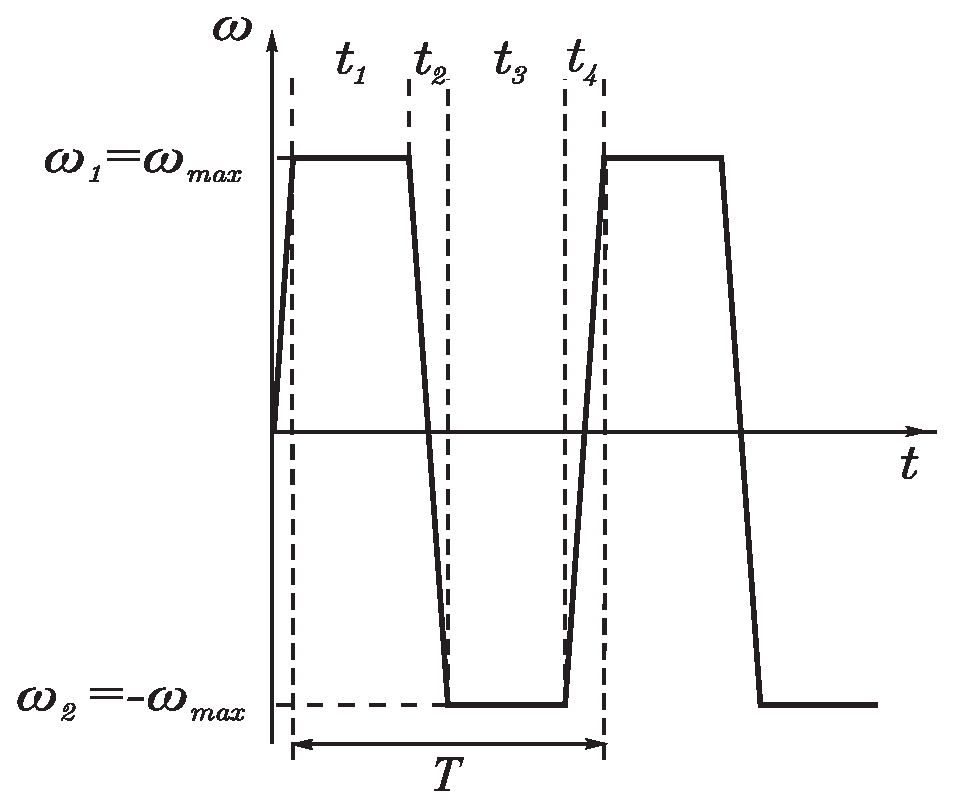
\includegraphics[width=0.4\linewidth]{ControlActionLine.eps}
	\caption{Зависимость угловой скорости ротора от времени}
	\label{ControlActionLine}
\end{figure}

%	\begin{equation}
%	\omega_r(t) =
%	\begin{cases}
%	
%	\omega_{r_{max}} & t \in \left[ nT;  nT + t_1 \right] ,\\
%	
%	\omega_{r_{max}}(10T(2n+1) - 20t - 1) & t \in \left[ nT + t_1;  nT + t_1+t_2 \right], \\
%	
%	-\omega_{r_{max}} & t \in \left[ nT + t_1+t_2;  nT + t_1+t_2+t_3 \right] ,\\
%	
%	\omega_{r_{max}}( 20t - 20T(n+1) + 1) &t \in \left[ nT + t_1 + t_2+t_3;  nT + t_1+t_2+t_3+t_4 \right] ,
%	
%	\end{cases}
%	\label{omegaRotorLine}
%	\end{equation}

\textit{Замечание. Фактически, на обмотки двигателя подавалось максимальное напряжение, у которого через равные промежутки времени изменялся знак на противоположный. Таким образом достигалась максимальная скорость вращения ротора с максимальным угловым ускорением для данного двигателя при имеющемся напряжении питания.}

Кадр с записи движения робота в бассейне представлен на рисунке~\ref{Frame1}. Как видно из рисунка, при данном управляющем воздействии робот движется вдоль прямой.

\begin{figure}[!ht]
	\centering
	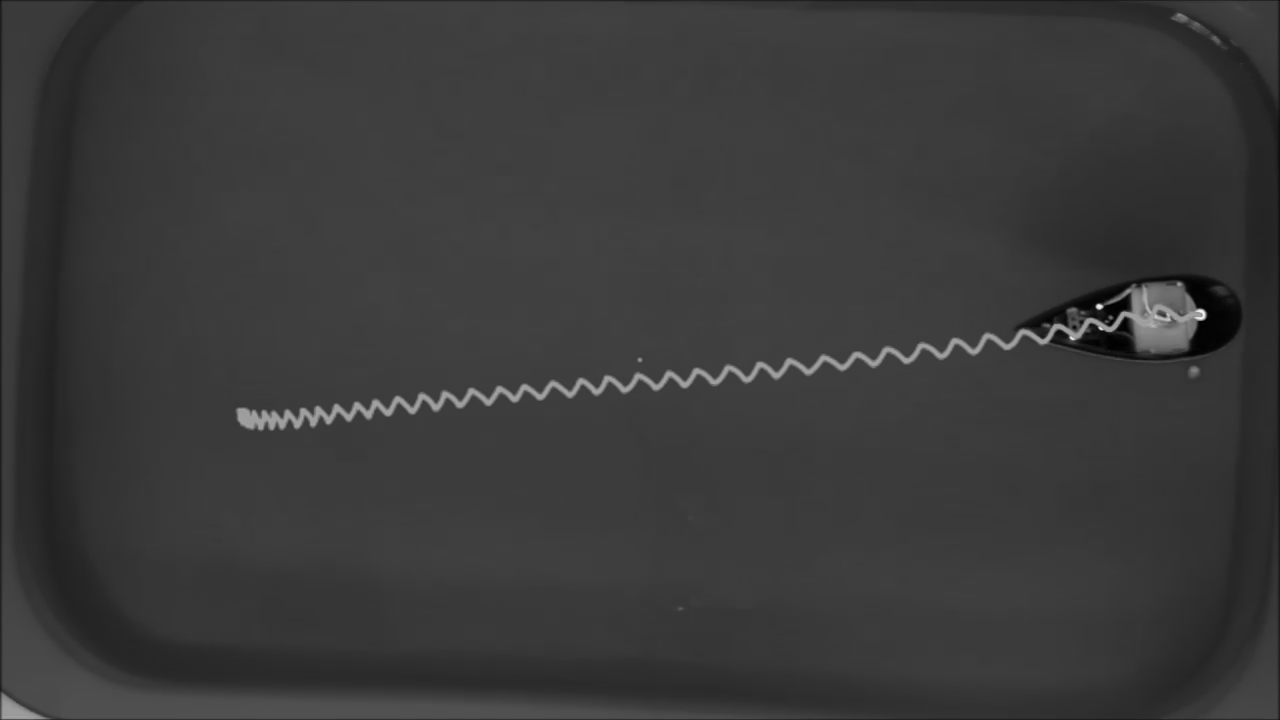
\includegraphics[width=0.7\linewidth]{Frame1.png}
	\caption{Кадр с записи движения робота в бассейне}
	\label{Frame1}
\end{figure}

%	Для моделирования задавалась функция углового ускорения в виде
%	
%	\begin{equation}
%	\ddot{\varphi} = A \cdot \cos\left( \frac{2\pi t}{T}\right) ^{m},
%	\label{ddPhi}
%	\end{equation}
%	
%	где А -- амплитуда углового ускорения, m -- нечетное число. Интегрируя данную функцию получаем зависимость угловой скорости от времени.





%	\begin{figure}[!ht]
%		\centering
%		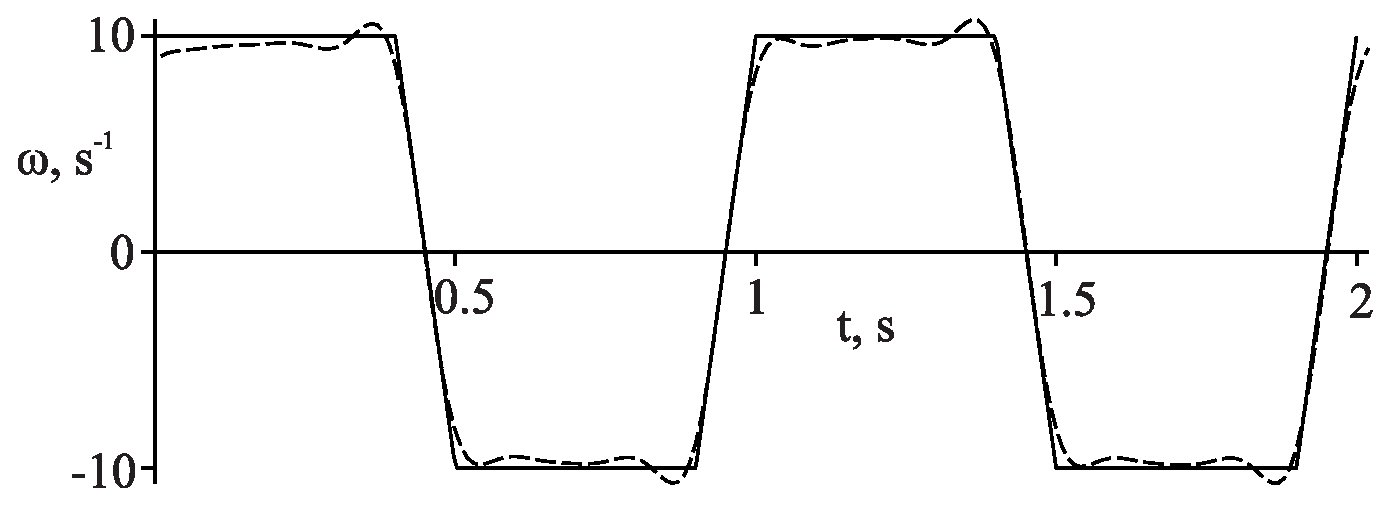
\includegraphics[width=\myVarFigs\linewidth]{OmegaT1Meandr.eps}
%		\caption{Зависимость угловой скорости ротора от времени при эксперименте (штриховая линия) и моделировании (сплошная линия) при $ T = 1 $}
%		\label{OmegaT1}
%	\end{figure}
%			
%	\begin{figure}[!ht]
%		\centering
%		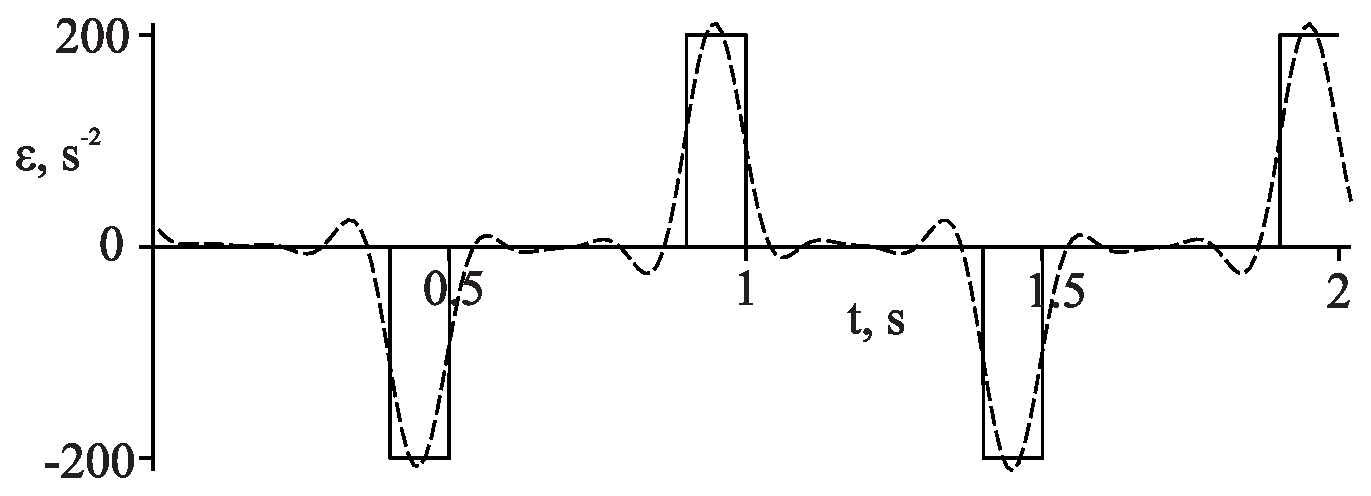
\includegraphics[width=\myVarFigs\linewidth]{EpsilonT1Meandr.eps}
%		\caption{Зависимость углового ускорения ротора от времени при эксперименте (штриховая линия) и моделировании (сплошная линия) при $ T = 1 $}
%		\label{EpsilonT1}
%	\end{figure}




Для движения по прямой были проведены эксперименты при $ T = 1, 2, 3, 4 $ секунды.

%	Сравнивая полученные значения с результатом моделирования можно сказать, что поперечная составляющая перемещения и скорости $ y(t) , \dot{y}(t) $ по частоте и форме совпадают достаточно хорошо во всех проведенных экспериментах
%	%(см. рисунки~\ref{y(t)T1},~\ref{dy(t)T1} для управляющего воздействия $ \omega_r(t) $ при $ T = 1 $)
%	.	Экспериментальная амплитуда несколько превышает расчетные значения.

%	\begin{figure}[!h]
%		\centering
%		\includegraphics[width=\myVarFigs\linewidth]{y(t)T1.eps}
%		\caption{Зависимость поперечной координаты робота от времени при эксперименте (штриховая линия) и моделировании (сплошная линия) при $ T = 1 $}
%		\label{y(t)T1}
%	\end{figure}
%
%	\begin{figure}[!h]
%		\centering
%		\includegraphics[width=\myVarFigs\linewidth]{dy(t)T1.eps}
%		\caption{Зависимость поперечной скорости робота от времени при эксперименте (штриховая линия) и моделировании (сплошная линия) при $ T = 1 $}
%		\label{dy(t)T1}
%	\end{figure}

%	Угловое перемещение и угловая скорость робота относительно вертикальной оси ведут себя аналогично: совпадают по форме и частоте, не совпадают по амплитуде, причем, амплитуда этих величин в эксперименте отличается в 2-4 раза от расчетной
%(см. рисунки ~\ref{phi(t)T1},~\ref{dphi(t)T1} для управляющего воздействия $ \omega_r(t) $ при $ T = 1 $).

%	\begin{figure}[!ht]
%		\centering
%		\includegraphics[width=\myVarFigs\linewidth]{phi(t)T1.eps}
%		\caption{Зависимость угла поворота робота вокруг вертикальной оси от времени при эксперименте (штриховая линия) и моделировании (сплошная линия) при $ T = 1 $}
%		\label{phi(t)T1}
%	\end{figure}
%
%	\begin{figure}[!ht]
%		\centering
%		\includegraphics[width=\myVarFigs\linewidth]{dphi(t)T1.eps}
%		\caption{Зависимость скорости поворота робота вокруг вертикальной оси от времени при эксперименте (штриховая линия) и моделировании (сплошная линия) при $ T = 1 $}
%		\label{dphi(t)T1}
%	\end{figure}

%	Продольная скорость является наименее предсказуемой, что сказывается и на продольном перемещении
%	%(см. рисунки ~\ref{x(t)T1},~\ref{dx(t)T1}
%	для управляющего воздействия $ \omega_r(t) $ при $ T = 1 $). За один период $ T $ в эксперименте у продольной скорости наблюдаются колебания с удвоенной частотой. В расчетах эти колебания присутсвуют, но имеют значительно меньшую амплитуду. Так же видно, что в эксперименте продольная скорость быстрее выходит на среднюю постоянную величину, чем в расчетах. Подобная картина характерна для всех экспериментов.

%	\begin{figure}[!ht]
%		\centering
%		\includegraphics[width=\myVarFigs\linewidth]{x(t)T1mod.eps}
%		\caption{Зависимость продольной координаты робота от времени при эксперименте (штриховая линия) и моделировании (сплошная линия) при $ T = 1 $}
%		\label{x(t)T1}
%	\end{figure}
%	
%	\begin{figure}[!ht]
%		\centering
%		\includegraphics[width=\myVarFigs\linewidth]{dx(t)T1.eps}
%		\caption{Зависимость продольной скорости робота от времени при эксперименте (штриховая линия) и моделировании (сплошная линия) при $ T = 1 $}
%		\label{dx(t)T1}
%	\end{figure}

На рисунке~\ref{AllTrajectories} представлены экспериментальные и расчетные траектории движения при различных управляющих воздействиях. Так же схематично обозначена ориентация робота в начальный и конечный моменты времени. Время моделирования и экспериментов для всех тестов составило 40 секунд (вследствие ограниченного размера бассейна).

\begin{figure}[!ht]
	\centering
	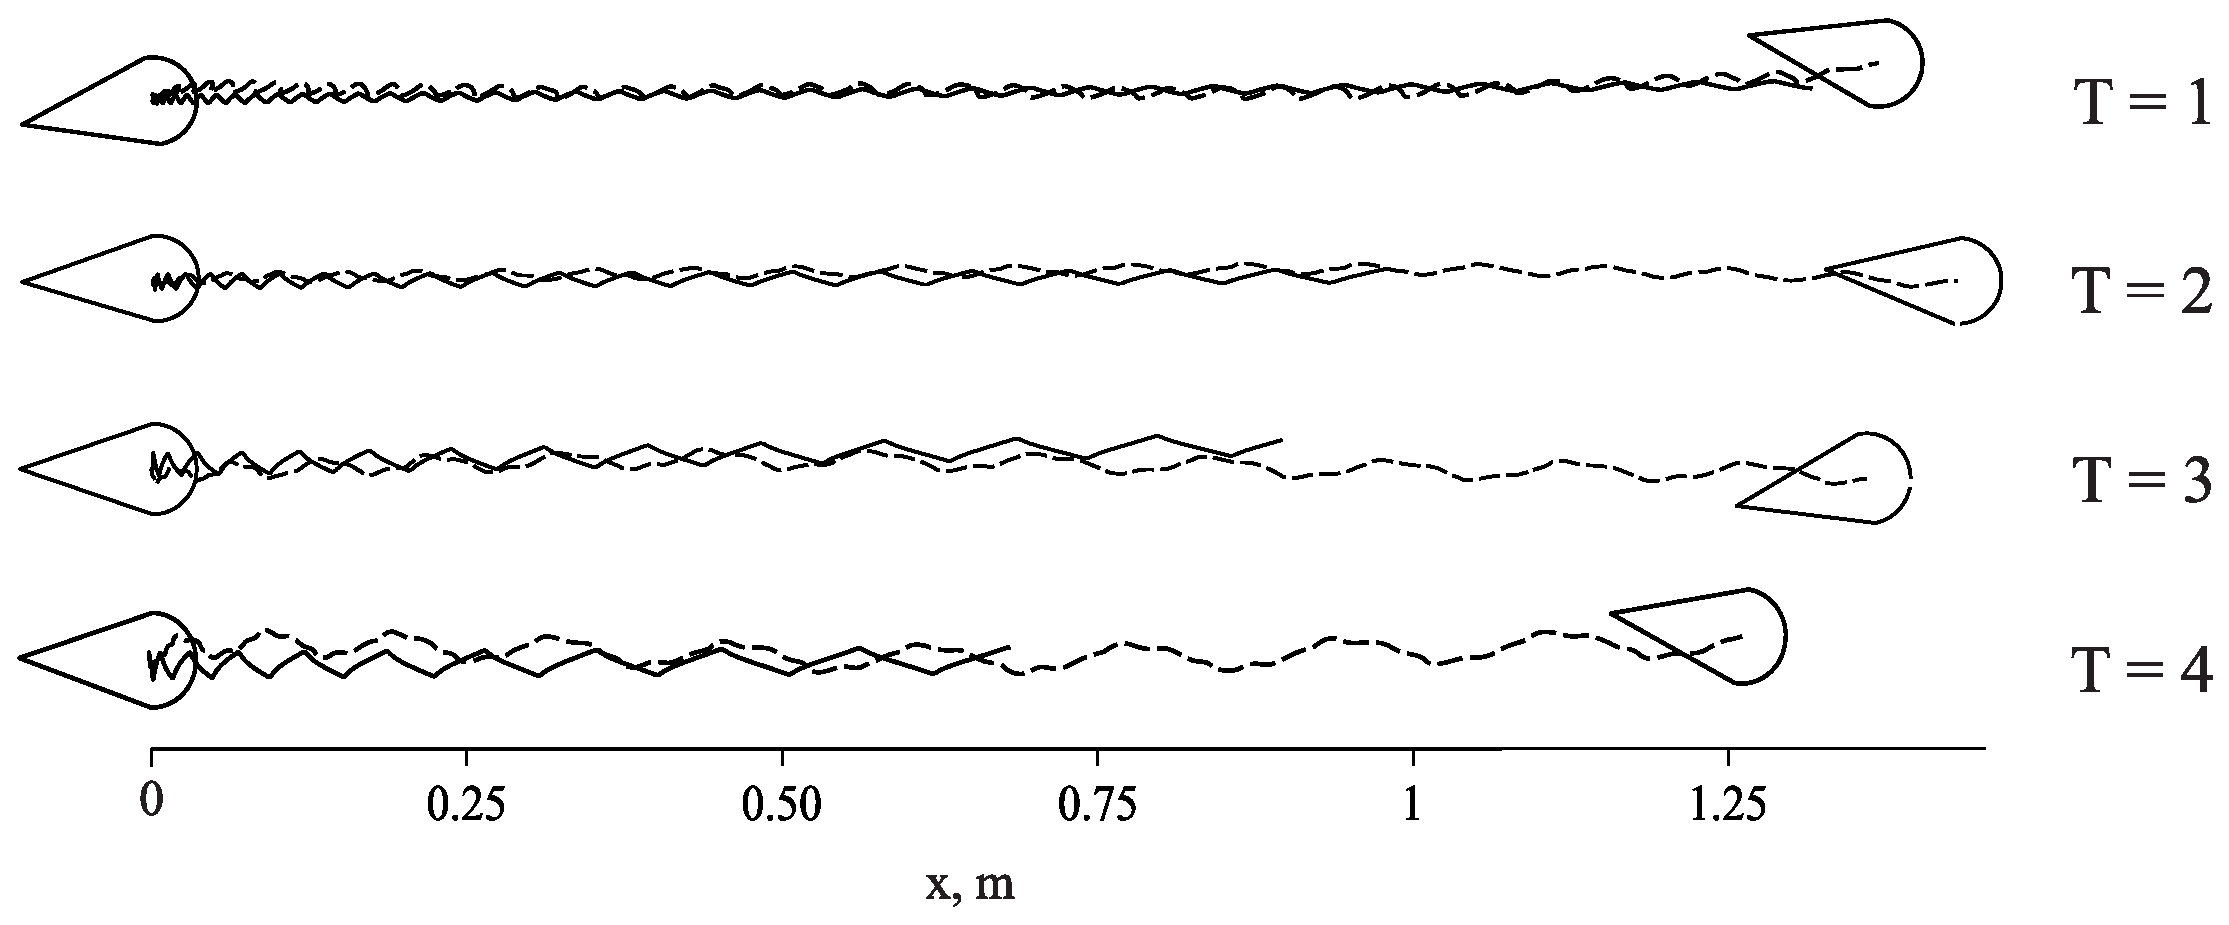
\includegraphics[width=0.8\linewidth]{AllTrajectories_new.eps}
	\caption{Траектории движения робота при  $ \omega_1 = \omega_{max} $, $ \omega_2 = -\omega_{max} $ и различных  управляющих воздействиях. Пунктирной линией обозначены траектории, полученные по результатам численного моделирования, сплошной -- экспериментальные траектории.}
	\label{AllTrajectories}
\end{figure}

Зависимость скорости движения робота от периода управляющего воздействия в рамках данных исследований не очевидна, возможно из-за ограниченных размеров бассейна. Наилучшее количественное согласование результатов моделирования с экспериментом получено при $T = 1$ c. Именно по этим экспериментальным данным проводилось вычисление коэффициентов в главе~\ref{ch:ch6}. Отклонение результатов моделирования от экспериментальных данных для других значений периода управляющего воздействия возможно минимизировать при уточнении значений коэффициентов модели для соответствующих условий эксперимента.

%Одним из объяснений несоответсвия является не точное совпадение формы углового ускорения в моделировании и при эксперименте.	На рисунке~\ref{OmegaT1EpsilonT1} для сравнения приведены аналитические (используемые при моделировании) и экспериментальные графики угловой скорости и углового ускорения ротора  при $ T = 1 $ cекунда. Видно, что графики для моделирования не полностью повторяют реальные зависимости, что приводит к неточностям в расчетах траектории.

%\begin{figure}[!ht]
%	\begin{minipage}[h]{0.5\linewidth}
%		\center{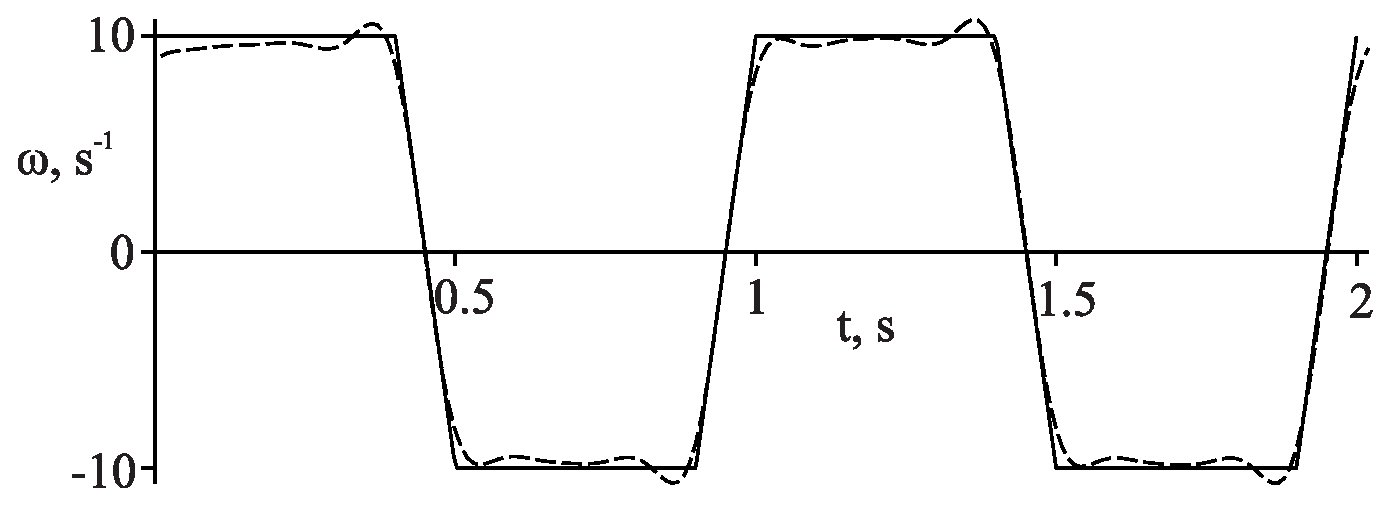
\includegraphics[width=0.9\linewidth]{OmegaT1Meandr.eps} \\ a}
%	\end{minipage}
%	\hfill
%	\begin{minipage}[h]{0.5\linewidth}
%		\center{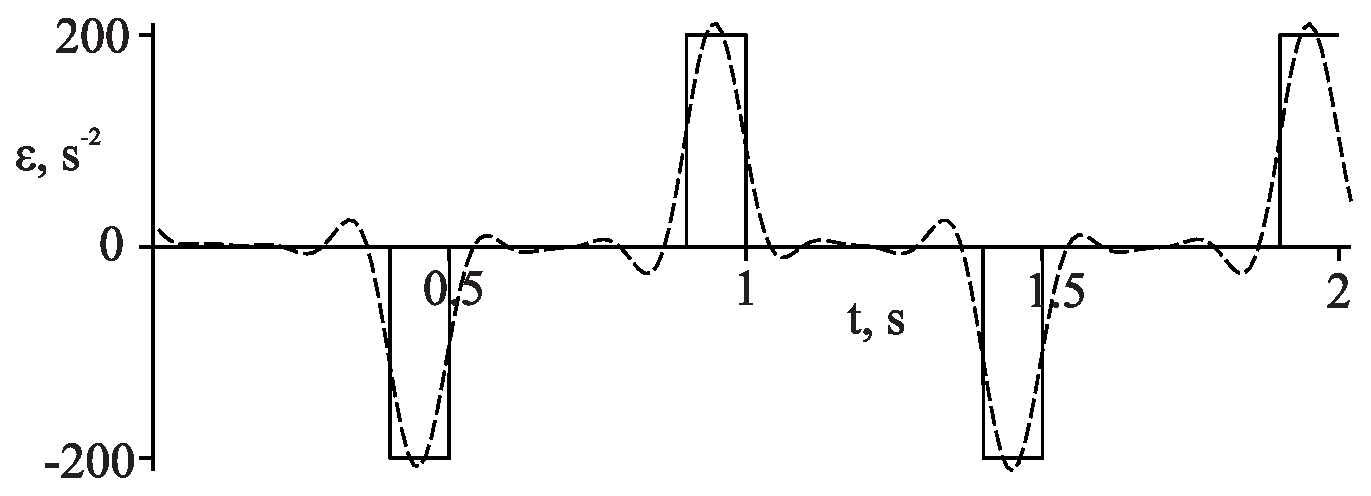
\includegraphics[width=0.9\linewidth]{EpsilonT1Meandr.eps} \\ b}
%	\end{minipage}
%	\caption{Зависимость угловой скорости ротора (a) и углового ускорения ротора (b) от времени при эксперименте (штриховая линия) и моделировании (сплошная линия)}
%	\label{OmegaT1EpsilonT1}
%\end{figure}


%На графиках видно, что с увеличением значения периода $ T $ расчетное перемещение по оси $ x $ показывает меньшую величину, а реальное перемещение отличия имеет небольшие. Можно сделать вывод, что траектории полученные в эксперименте от периода управляющих импульсов зависят не сильно, при изменении $ T $ в 4 раза, робот перемещается примерно на одно расстояние по оси $ x $.
%При данных управляющих воздействиях максимальное расстояние по оси $ x $ робот преодолевает при $ T = 2 $ секунды, с увеличением $ T $ наблюдается нисходящая зависимость.

Для несимметричных управляющих воздействий, например при смещении угловой скорости на величину $\omega_0$ (см. рис.~\ref{DifferentAmp}a), и сохранении равенств интервалов $t_1=t_3$, $t_2=t_4$  робот также двигается вдоль прямой.  Для наглядности сравнения экспериментов влияния смещения на характер траектории соотношение угловых скоростей оставалось постоянным $ \omega_1 - \omega_2 = const$.  На рис.~\ref{DifferentAmp}b приведены соответствующие траектории движения робота, из которых видно что робот двигался в среднем прямолинейно, но в различных направлениях. Причем изменение направления происходит в начале движения, а угол поворота зависит от сдвига управления $\omega_0$. 
%Видео файлы подтверждающие полученные нами результаты можно найти по ссылке  \textcolor{red}{ссылка видео 3 эксперимента с несимметричным управлением}.

%При использовании несимметричного управляющего воздействия, а именно его смещении, то есть вращении ротора по часовой и против часовой стрелки с разными угловыми скоростями, как по результатам экспериментов, так и по результатам моделирования получены результаты противоположные выводам в работе \cite{Pollard_Tallapragada_2016}.  Примеры исследуемых управлений при $ t_2=t_4=0.1 $ $ t_1=t_3=0.9 $, $T = 2$ приведены на рисунке~\ref{DifferentAmp}a. Для возможности сравнения результатов в данных экспериментах разница угловых скоростей обеспечивалась постоянной $ \omega_1 - \omega_2 = const$.

%Несмотря на несимметричность управления, робот плыл вдоль прямой во всех трех экспериментах (см. рисунок~\ref{DifferentAmp}b), хотя в работе \cite{Pollard_Tallapragada_2016} робот поворачивался, и начинал плыть вдоль окружности.  Несимметричность управления в наших экспериментах приводит только к повороту робота в момент начала движения, причем угол поворота зависит от несимметричности управления. Видео файлы подтверждающие полученные нами результаты можно найти по ссылке  \textcolor{red}{ссылка видео 3 эксперимента с несимметричным управлением}.

%	\begin{figure}[!ht]
%		\begin{minipage}[h]{0.3\linewidth}
%			\center{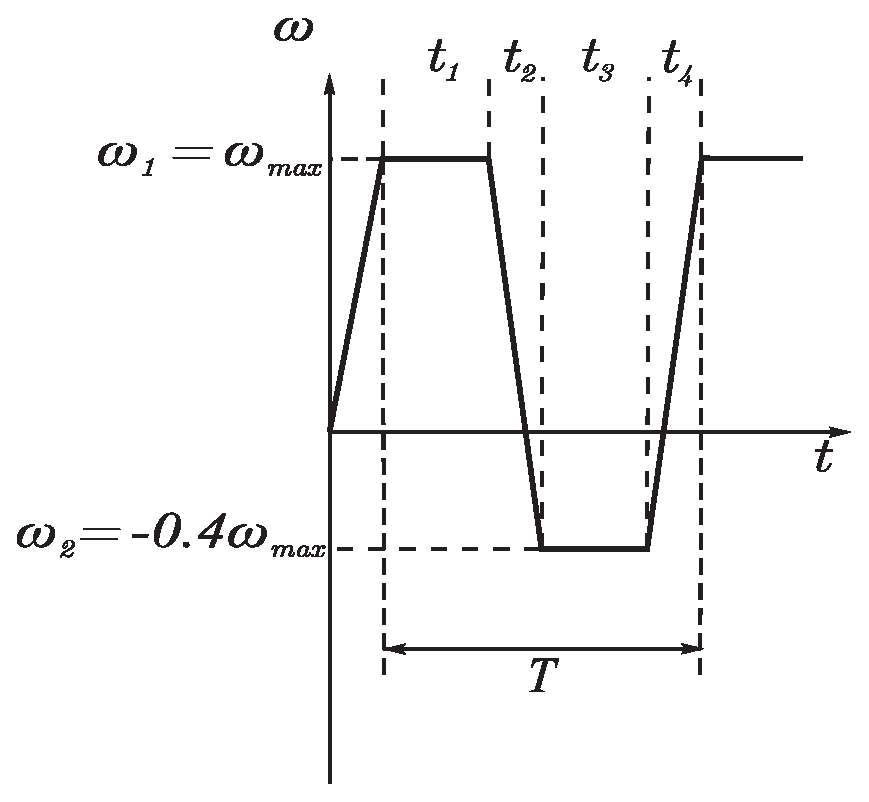
\includegraphics[width=0.9\linewidth]{ControlActionDifferentAmp1_line.eps} \\ a}
%		\end{minipage}
%		\hfill
%		\begin{minipage}[h]{0.3\linewidth}
%			\center{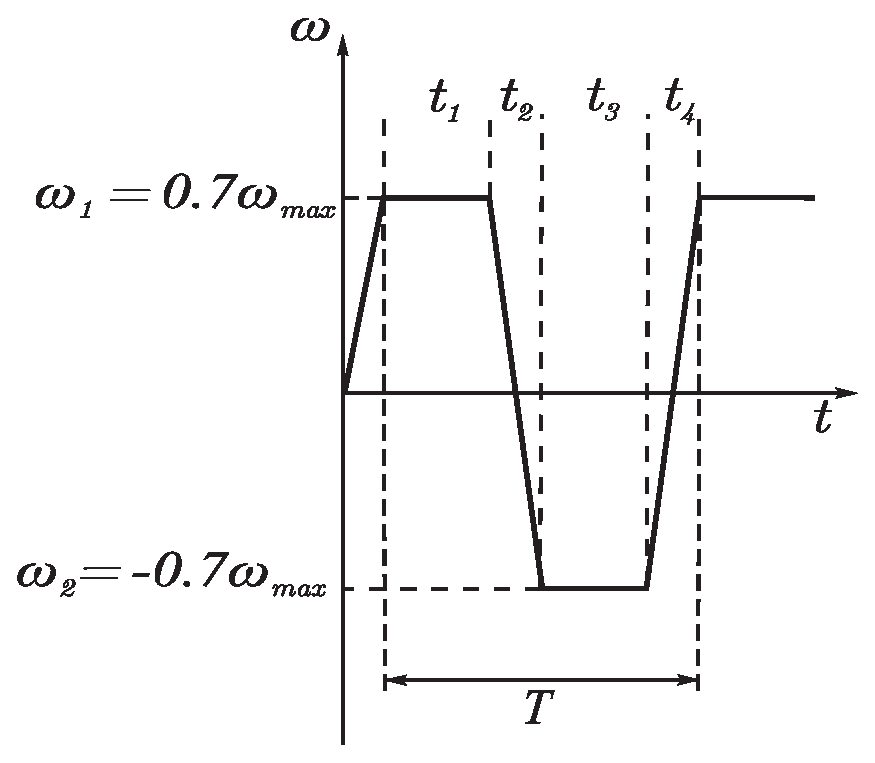
\includegraphics[width=0.9\linewidth]{ControlActionDifferentAmp2_line.eps} \\ b}
%		\end{minipage}
%		\hfill
%		\begin{minipage}[h]{0.3\linewidth}
%			\center{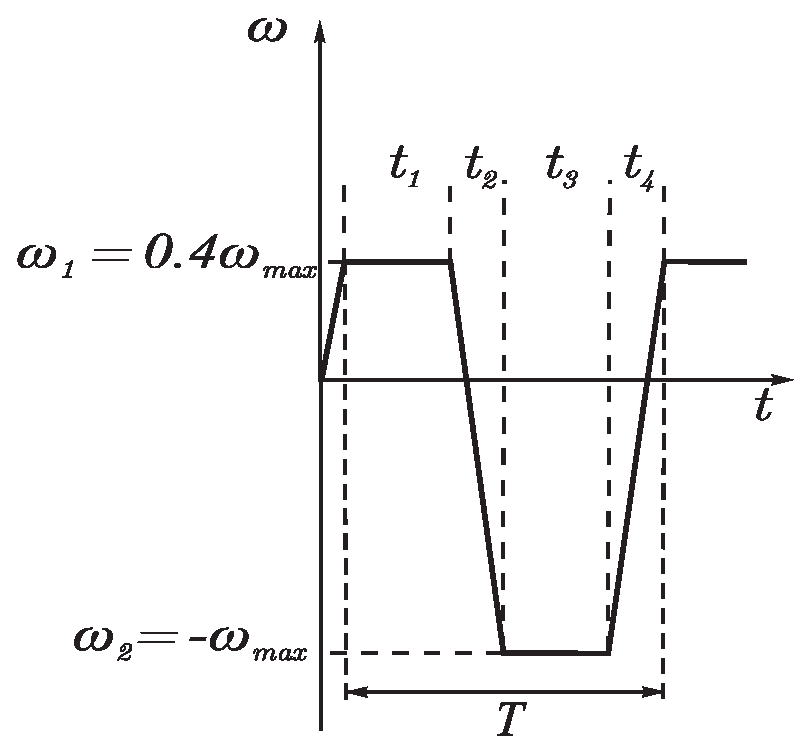
\includegraphics[width=0.9\linewidth]{ControlActionDifferentAmp3_line.eps} \\ c}
%		\end{minipage}
%		\caption{ \textcolor{red} { сделать три графика на одном рисунке, в одних осях, выделить также как траектории} Несиммтеричные упраляющие воздействия при $\omega_1 - \omega_2 = const$, \textcolor{red}{чем отличаются а,б,с И переделать рисунок $t_1 = t_3$ }}
%		\label{ControlActionDifferentAmp}
%	\end{figure}

%    \begin{figure}[!ht]
%		\centering
%		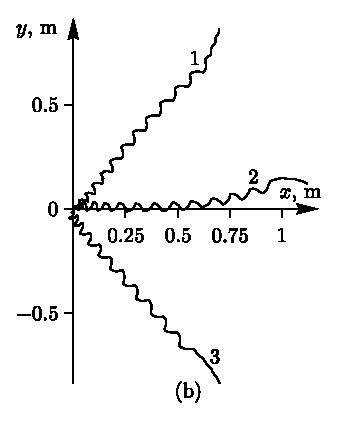
\includegraphics[width=0.35\linewidth]{Plots3.eps}
%		\caption{Траектории движения робота c изменением амплитуды угловой скорости при обеспечении разницы  $ \omega_1 - \omega_2 = const$. \textcolor{red} {Траектория 1 соответствует управлению с рисунка~\ref{ControlActionDifferentAmp}a, траектория 2 соответствует управлению с рисунка~\ref{ControlActionDifferentAmp}b, траектория 3 соответствует управлению с рисунка~\ref{ControlActionDifferentAmp}c}}
%		\label{TrajectoriesDifferentAmp}
%	\end{figure}

\begin{figure}[!ht]
	\begin{minipage}[h]{0.5\linewidth}
		\center{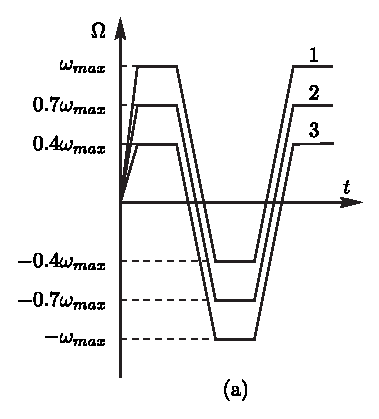
\includegraphics[height=0.9\linewidth]{ControlActionPlots3.eps} \\ }
	\end{minipage}
	\hfill
	\begin{minipage}[h]{0.5\linewidth}
		\center{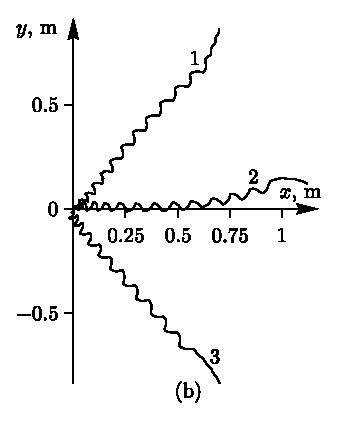
\includegraphics[height=0.9\linewidth]{Plots3.eps} \\ }
	\end{minipage}
	\caption{Несимметричные управляющие воздействия при $\omega_1 - \omega_2 = const$, $t_2 = t_4 = 0.1$, $t_1 = t_3 = 0.9$, $T = 2$ (a) и соответствующие им траектории движения водного робота (b).}
	\label{DifferentAmp}
\end{figure}

%\begin{figure}[!ht]
%	\centering
%	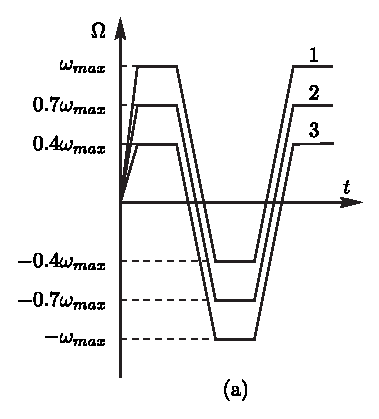
\includegraphics[width=1\linewidth]{ControlActionPlots3.eps}\hspace{20mm}
%	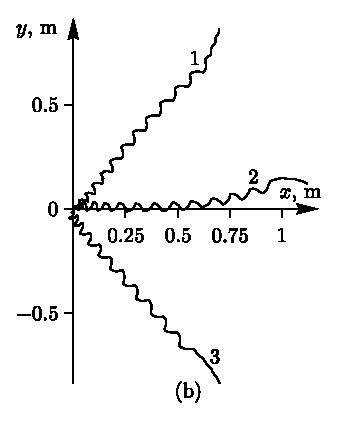
\includegraphics[width=1\linewidth]{Plots3.eps}
%	\caption{Несимметричные управляющие воздействия при $\omega_1 - \omega_2 = const$, $t_2 = t_4 = 0.1$, $t_1 = t_3 = 0.9$, $T = 2$ (a) и соответствующие им траектории движения водного робота (b).}
%	\label{DifferentAmp}
%\end{figure}

По результатам проведенных экспериментальных исследований можно сделать следующие выводы.
\begin{itemize}
	\item[-] Рассматриваемая теоретическая модель управляемого движения водного робота качественно правильно  описывает его движение вдоль прямой, которое реализуется симметричным управляющим воздействием.
	
	\item[-] Сдвиг управляющего воздействия $\Omega(t) \rightarrow \omega_0 + \Omega(t)$ не влияет на форму траектории, она остается прямой, но меняется направление движение.
	
	\item[-] Количественного согласования результатов моделирования и экспериментов можно достичь для конкретных тестов, проводя перерасчет коэффициентов под конкретные экспериментальные данные.
\end{itemize}



\subsection{Движение вдоль окружности}

Движение робота по траектории по форме близкой к окружности оказывается возможным, если в управляющем воздействии \eqref{omegaRotorGeneral} положить $t_1 \neq t_3$ и $t_2 = t_4$. То есть длительности вращения ротора в направлениях по часовой стрелке и против часовой стрелки различны. Типовая траектория движения робота при
\begin{gather}
t_3 = 10 t_1,\quad \omega_1 = \omega_{max},\quad \omega_2 = -\omega_{max},\quad t_2 = t_4 = 0.1~\text{с},\quad T = 3~\text{с}
\end{gather}
и результаты моделирования приведены на рис.~\ref{CircleTrajectory}a. На рис.~\ref{CircleTrajectory}b приведена графическая зависимость радиуса окружности, аппроксимирующей траекторию, от соотношения длительностей рассматриваемых интервалов $k_1 = t_3 / t_1$. Для построения аппроксимаций расчетных и экспериментальных данных использовался метод наименьших квадратов.

%При условии различий длительности интервалов, на которых происходит вращение с постоянной угловой скоростью по и против движения часовой стрелки, т.е. при $t_1 \neq t_3$ и прочих равных условиях $t_2 = t_4$,  робот  двигается вдоль траектории близкой по форме к окружности. Типовая траектория движения робота при  $t_3 = 10 t_1$, $ \omega_1 = \omega_{max} $; $ \omega_2 = -\omega_{max} $; $ t_2=t_4=0.1 $ с; $ T = 3 $ с, а также результаты моделирования приведены на рисунке \ref{CircleTrajectory}a. На рисунке \ref{CircleTrajectory}b приведена графическая зависимость радиуса окружности, полученного для аппроксимации траектории движения робота с помощью метода наименьших квадратов по экспериментальным данным с системы захвата движения, от соотношения длительностей рассматриваемых интервалов $ k_1 = t_3 / t_1 $.

\begin{figure}[!ht]
	\begin{minipage}[h]{0.3\linewidth}
		\center{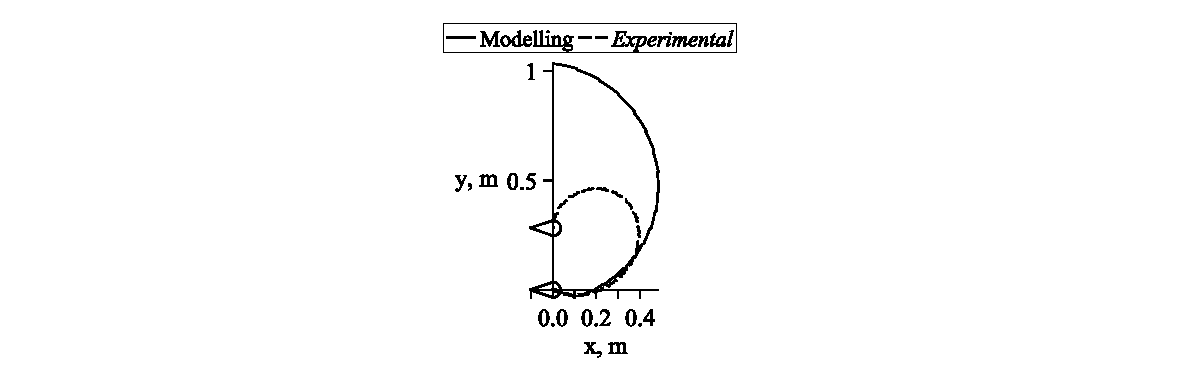
\includegraphics[width=0.8\linewidth]{xyCircleWmax.eps} \\ a}
	\end{minipage}
	\hfill
	\begin{minipage}[h]{0.7\linewidth}
		\center{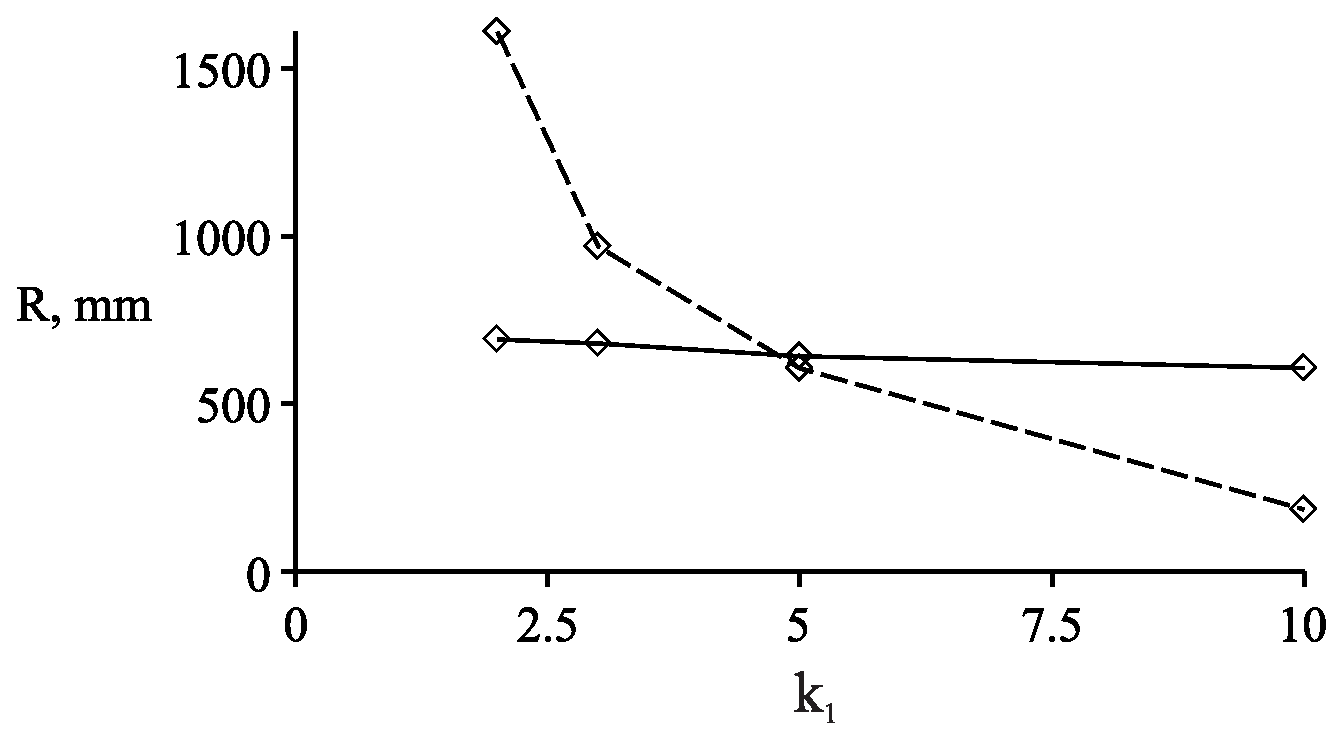
\includegraphics[width=0.9\linewidth]{kRDependence+Theor_T=3,W=max.eps} \\ b}
	\end{minipage}
	\caption{a) Траектория движения робота по окружности при эксперименте (штриховая линия) и моделировании (сплошная линия)  b) Зависимость радиуса траектории движения робота от $k_1 = \frac{t_3}{t_1}$ при эксперименте (штриховая линия) и моделировании (сплошная линия) построенная по экспериментам при $k_1 = 2,\ 3,\ 5,\ 10$ }
	\label{CircleTrajectory}
\end{figure}

%\begin{figure}[!ht]
%	\centering
%	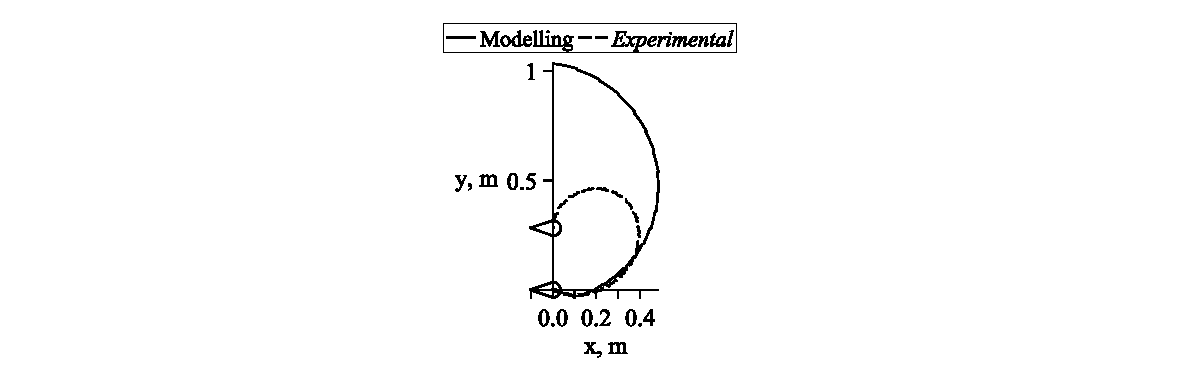
\includegraphics{xyCircleWmax.eps}
%	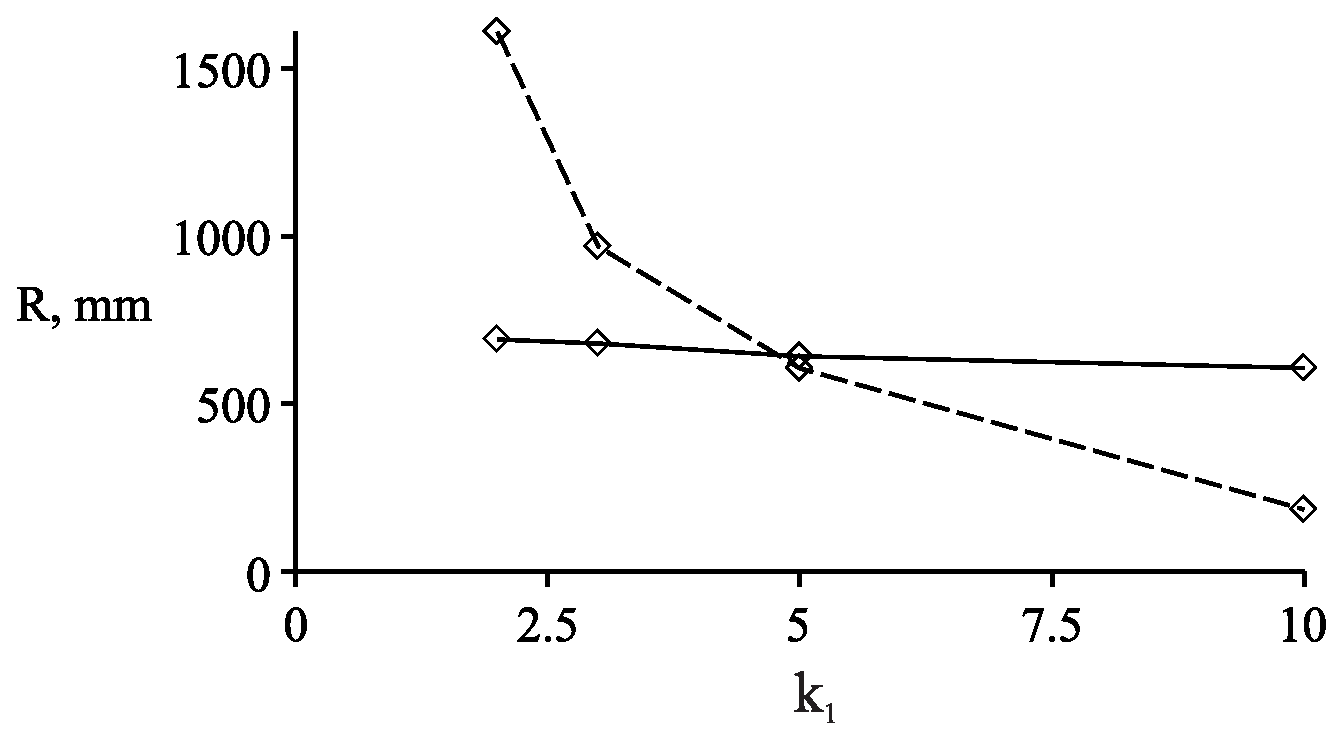
\includegraphics{kRDependence+Theor_T=3,W=max.eps}
%	\caption{a) Траектория движения робота по окружности при эксперименте (штриховая линия) и моделировании (сплошная линия)  b) Зависимость радиуса траектории движения робота от $k_1 = \frac{t_3}{t_1}$ при эксперименте (штриховая линия) и моделировании (сплошная линия) построенная по экспериментам при $k_1 = 2,\ 3,\ 5,\ 10$ }
%	\label{CircleTrajectory}
%\end{figure}

Форма расчетной и экспериментальной траектории качественно совпадают, но радиус окружности вдоль которой плывет робот при моделировании примерно в 2 -- 2.5 раза больше радиуса окружности, полученной в экспериментах.

Из рис.~\ref{CircleTrajectory}b видно, что радиус траекторий, полученных при моделировании, незначительно уменьшается при увеличении $k_1$. Для траекторий, полученных в эксперименте, при увеличении $k_1$ в 4 раза, радиус траектории уменьшается более чем в 4 раза.

%Из рисунка \ref{CircleTrajectory}b видно, что радиус окружности при моделировании уменьшается при увеличении $ k_1 $, но не существенно. В экспериментах зависимость более явная.
При данном управлении на практике минимальный радиус окружности, вдоль которой происходит движение, ограничен и определятся минимальным значением $t_3$ (или $t_1$ при движении вдоль окружности по часовой стрелке), которое определяется моменто-инерционными характеристиками системы  "двигатель -ротор". Для рассматриваемой нами модели робота минимальное значение радиуса окружности составило 185 мм.

Движения водного робота вдоль окружности меньшего радиуса поворота, а также более быстрого движения вдоль траектории можно добиться при изменении интервалов времени, соответствующих разгону и торможению, задаваемых величинами $t_2, t_4$ и определяющих угловое ускорение вращения ротора. Графическое представление типового управления при $t_2 \neq t_4$ приведено на рис.~\ref{ControlActionOur}a. На рис.~\ref{ControlActionOur}b представлены экспериментальная и расчетная траектории движения робота при данном управляющем воздействии для следующих значений
\begin{gather}
T=5,\quad t_4 = 0.1,\quad t_2 = 3,\quad \omega_1 = \omega_{max},\quad \omega_2 = -\omega_{max}.
\end{gather}

\begin{figure}[!ht]
	\begin{minipage}[h]{0.5\linewidth}
		\center{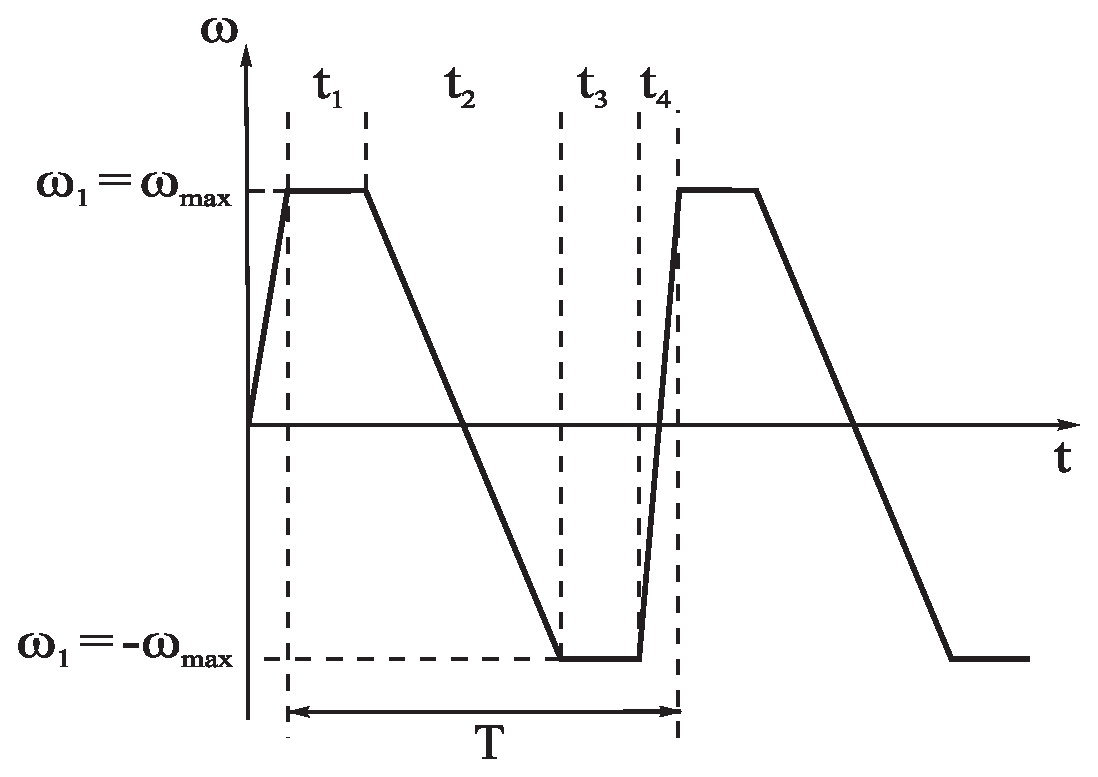
\includegraphics[width=0.9\linewidth]{ControlActionOur1.eps} \\ a}
	\end{minipage}
	\hfill
	\begin{minipage}[h]{0.5\linewidth}
		\center{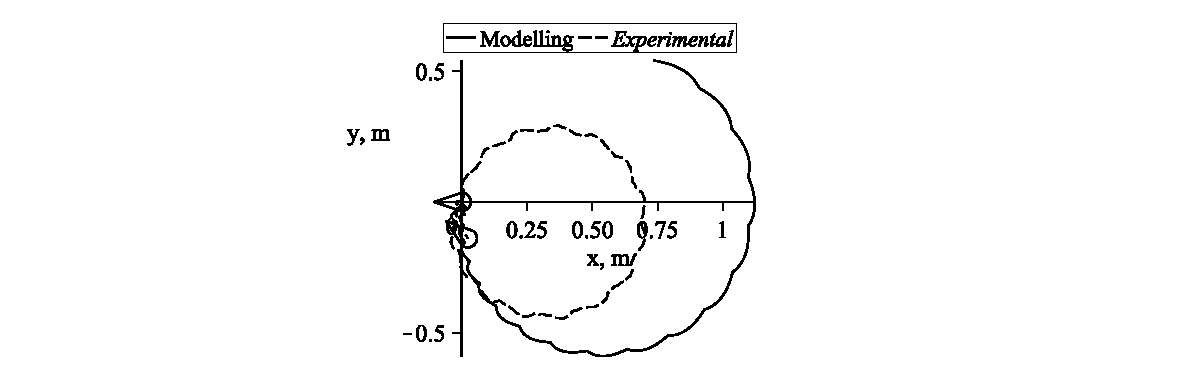
\includegraphics[width=0.8\linewidth]{xyCircleOur.eps} \\ b}
	\end{minipage}
	\caption{а) зависимость угловой скорости вращения ротора от времени при $t_2  \neq t_4$, b) типовая траектория движения робота вдоль окружности при $T = 5$, $t_1 = t_3 = 0.95$, $t_2 = 3$, $t_4 = 0.1$, $\omega_1 = \omega_{max}$, $\omega_2 = -\omega_{max}$ в эксперименте (штриховая линия) и моделировании (сплошная линия)}
	\label{ControlActionOur}
\end{figure}

%\begin{figure}[!ht]
%	\centering
%	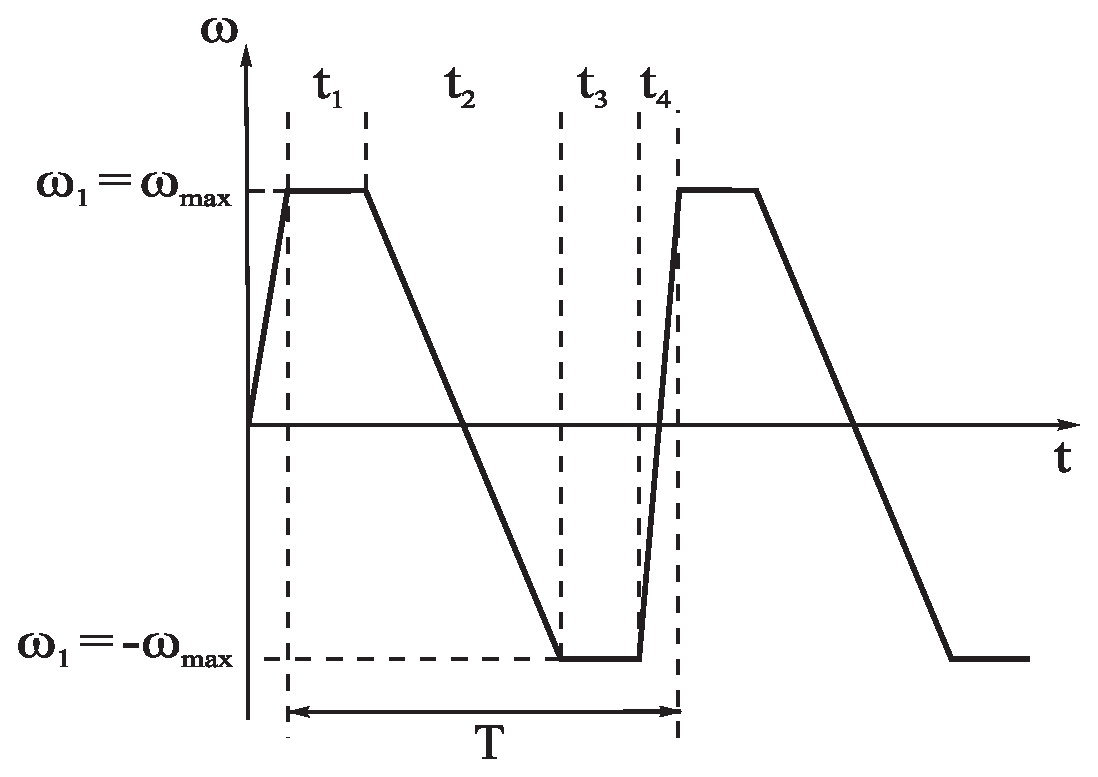
\includegraphics{ControlActionOur1.eps}\hspace{10mm}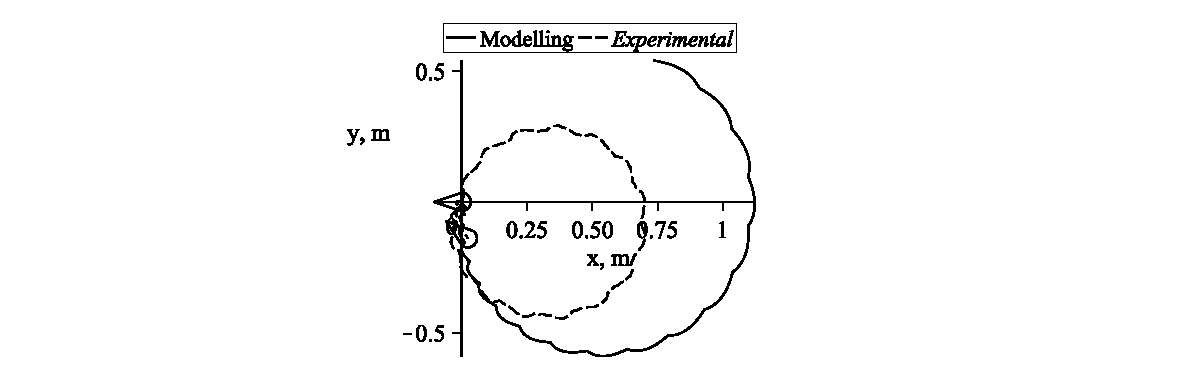
\includegraphics{xyCircleOur.eps}
%	\caption{а) зависимость угловой скорости вращения ротора от времени при $t_2  \neq t_4$, b) типовая траектория движения робота вдоль окружности при $T = 5$, $t_1 = t_3 = 0.95$, $t_2 = 3$, $t_4 = 0.1$, $\omega_1 = \omega_{max}$, $\omega_2 = -\omega_{max}$ в эксперименте (штриховая линия) и моделировании (сплошная линия)}
%	\label{ControlActionOur}
%\end{figure}

На рис.~\ref{nROur} приведены экспериментальная и расчетная зависимости радиуса траектории движения робота от коэффициента $k_2 = t_2 / t_4$. Эксперименты проводились для $k_2 = 10,\ 20,\ 30,\ 40$.

\begin{figure}[!ht]
	\centering
	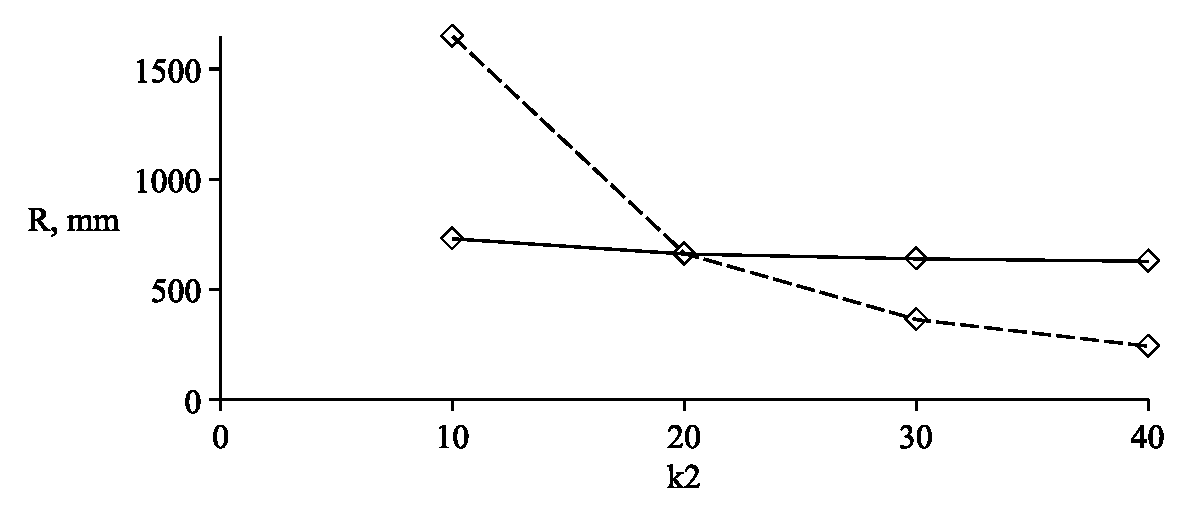
\includegraphics[width=0.8\linewidth]{nROur.eps}
	\caption{Теоретическая (сплошная линия) и экспериментальная (штриховая линия) зависимости радиуса траектории движения робота от $k_2$ при $\omega_1 = \omega_{max} $; $ \omega_2 = -\omega_{max} $; $ t_1=t_3 $; $ t_4=0.1 $ секунды; $ T = 5 $ секунд}
	\label{nROur}
\end{figure}

Качественно при увеличении неравенства продолжительности интервалов $t_2$, $t_4$ радиус окружности, вдоль которой движется робот, уменьшается, однако, в эксперименте данная зависимость имеет нелинейный и более выраженный характер.

При $k_2 = 20$ радиусы окружностей, вдоль которой плывет робот, полученные при моделировании и в эксперименте совпадают. Это объясняется тем, что при моделировании использовались значения   коэффициентов, полученные из экспериментальных данных, соответствующих движению вдоль прямой.

Выделим основные результаты данной серии экспериментальных исследований.

\begin{itemize}
	\item [-] Рассматриваемая теоретическая модель управляемого движения водного робота качественно правильно  описывает его движение вдоль окружности, которое реализуется асимметричным на периоде управляющим воздействием.
	
	\item [-] На размер и форму траектории движения влияет асимметрия управляющего воздействия на его периоде. Изменение направления движения -- поворот, может быть реализован либо при изменении продолжительности интервала вращения с постоянной угловой скоростью, либо вращением ротора по и против часовой стрелки с различными угловыми ускорениями.
	
	\item [-] Количественного согласования результатов моделирования и экспериментов, как и в при движении вдоль прямой, можно достичь для конкретных тестов, проводя перерасчет коэффициентов под конкретные экспериментальные данные, полученные при движении вдоль окружности.
	
\end{itemize}

\subsection{Движение вдоль сложных траекторий}

При комбинировании рассматриваемых управлений, обеспечивающих движение вдоль прямой и окружности, можно реализовать движение вдоль сложных траекторий. На рис.~\ref{Slalom}a приведен пример управляющего воздействия с тремя характерными управлениями: движение вдоль прямой, поворот направо, поворот налево.   Траектории полученные в эксперименте и моделировании приведены на рис.~\ref{Slalom}b.

\begin{figure}[!ht]
	\begin{minipage}[h]{0.5\linewidth}
		\center{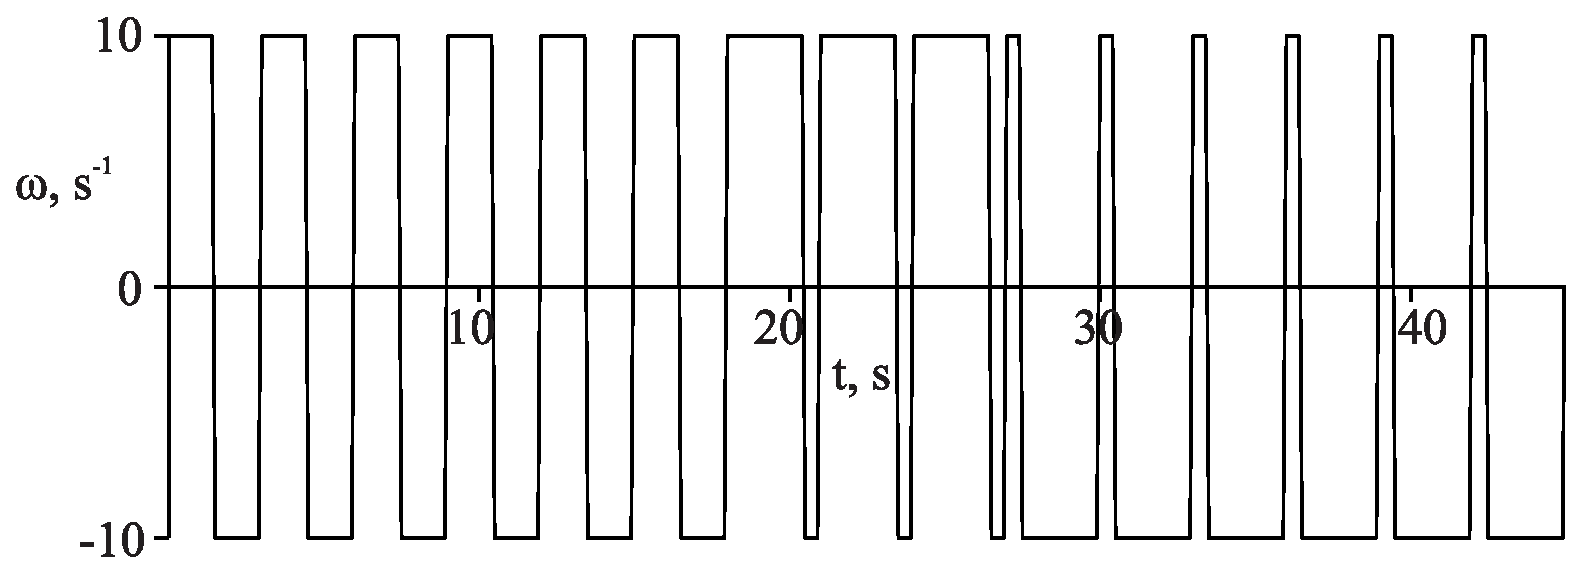
\includegraphics[width=0.9\linewidth]{ControlActionComplexTr.eps} \\ a}
	\end{minipage}
	\hfill
	\begin{minipage}[h]{0.5\linewidth}
		\center{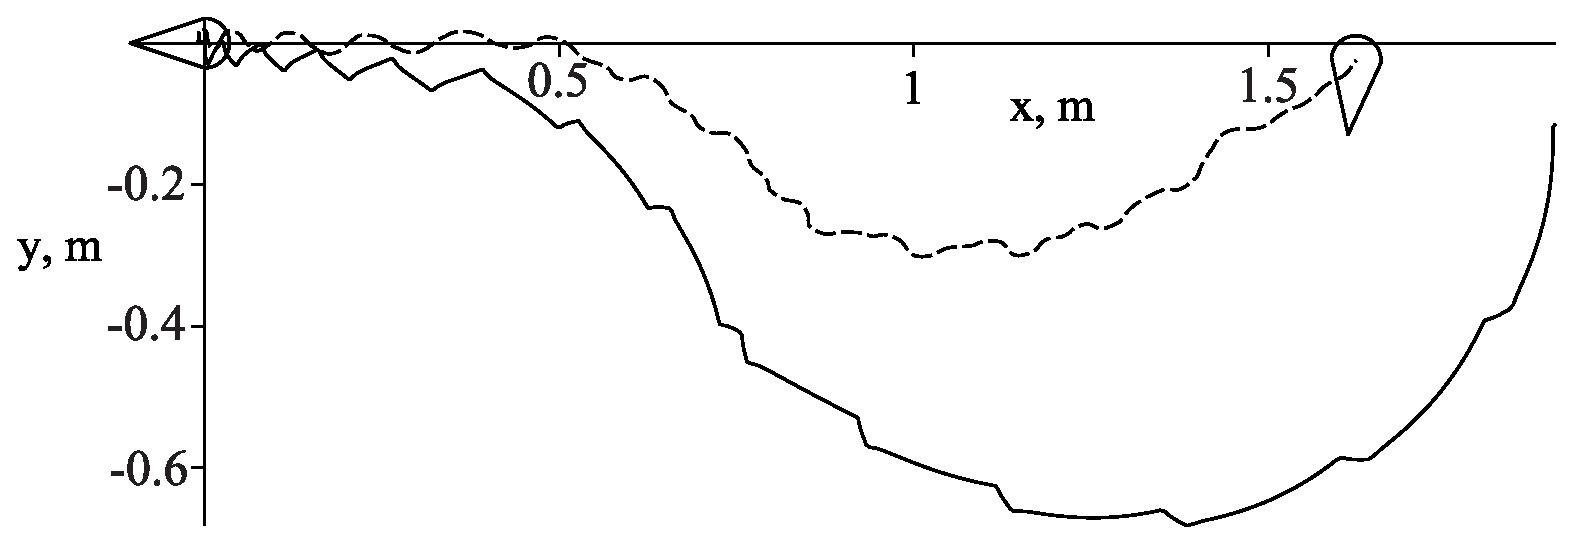
\includegraphics[width=0.9\linewidth]{ComplexTr.eps} \\ b}
	\end{minipage}
	\caption{Управления для реализации сложного движения (a) и соответствующая траектория движения (b)  при эксперименте (штриховая линия) и моделировании (сплошная линия)}
	\label{Slalom}
\end{figure}

%\begin{figure}[!ht]
%	\centering
%	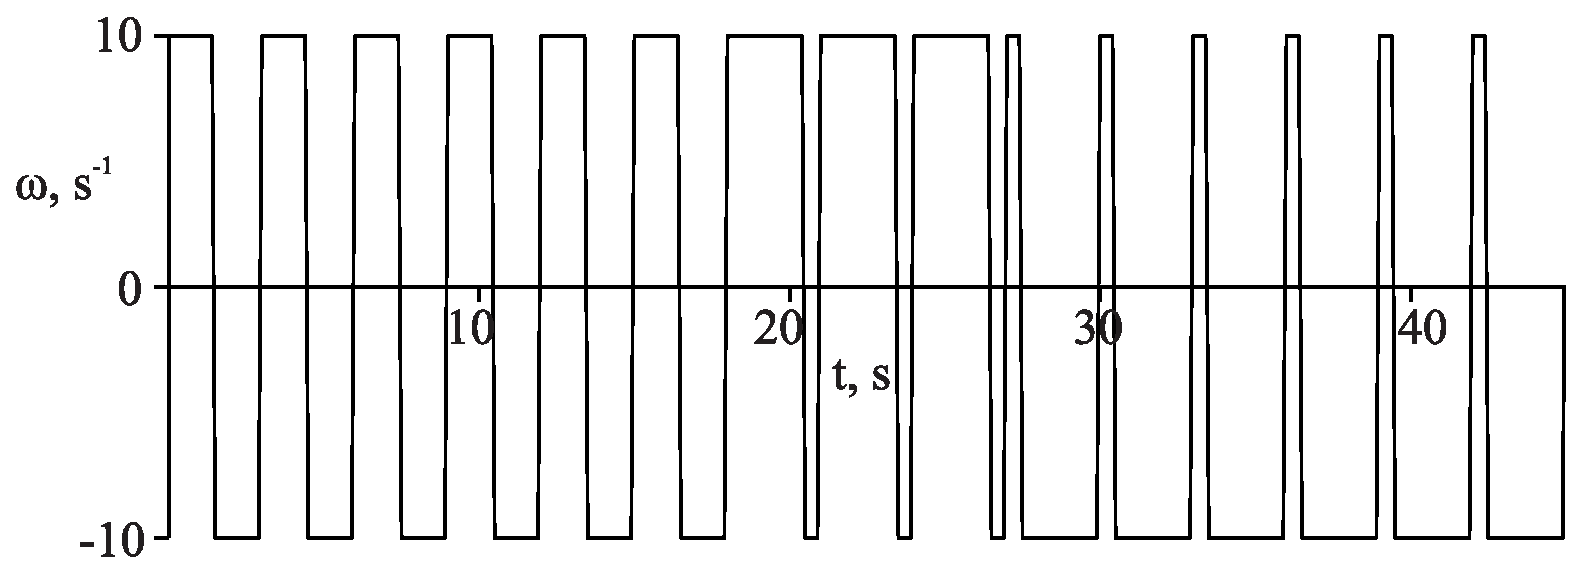
\includegraphics{ControlActionComplexTr.eps}\hspace{5mm}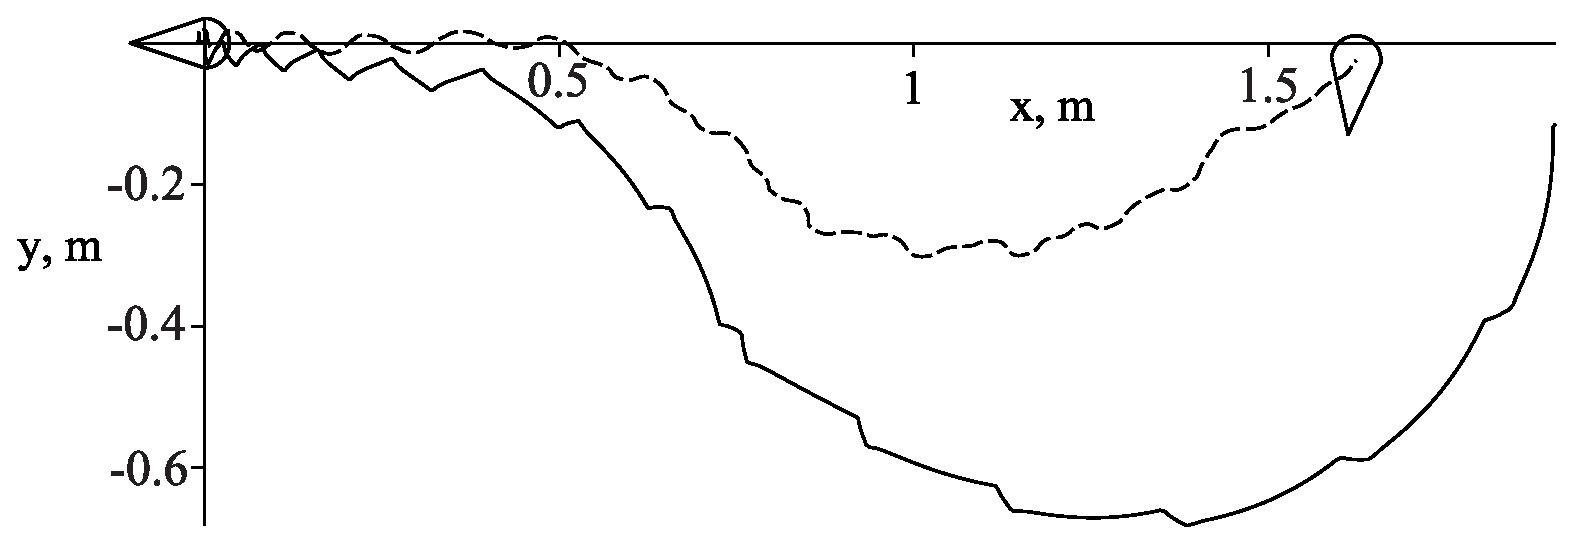
\includegraphics{ComplexTr.eps}
%	\caption{Управления для реализации сложного движения (a) и соответствующая траектория движения (b)  при эксперименте (штриховая линия) и моделировании (сплошная линия)}
%	\label{Slalom}
%\end{figure}

Полученные результаты также подтверждают возможность теоретической модели качественно описать движение водного робота, а также возможность формирования управления вдоль сложных криволинейных траектории, разбивая их на характерные участки, для которых можно сформировать базовые управления -- гейты. 

\subsection{Выводы по главе}

Одной из причин отклонения результатов численного моделирования от результатов натурных экспериментов является то, что при моделировании для всех серий экспериментов использовались коэффициенты сопротивления и присоединенных масс, рассчитанные на основании экспериментальных  данных, полученных при симметричном управляющем воздействии с $T = 1$ c. При других параметрах управления характер движения меняется существенно, что требует уточнения значений данных коэффициентов. Пользуясь экспериментальным подбором коэффициентов для различных гейтов, можно существенно улучшить получаемые результаты.

Еще одной причиной несогласованности теории и эксперимента является не точное совпадение формы углового ускорения в моделировании и при эксперименте. На рис.~\ref{OmegaT1EpsilonT1} для сравнения приведены аналитические (используемые при моделировании) и экспериментальные графики угловой скорости и углового ускорения ротора при $ T = 1 $ c. Видно, что графики для моделирования не полностью повторяют реальные зависимости, что приводит к неточностям в расчетах траектории.

\begin{figure}[!ht]
	\begin{minipage}[h]{0.5\linewidth}
		\center{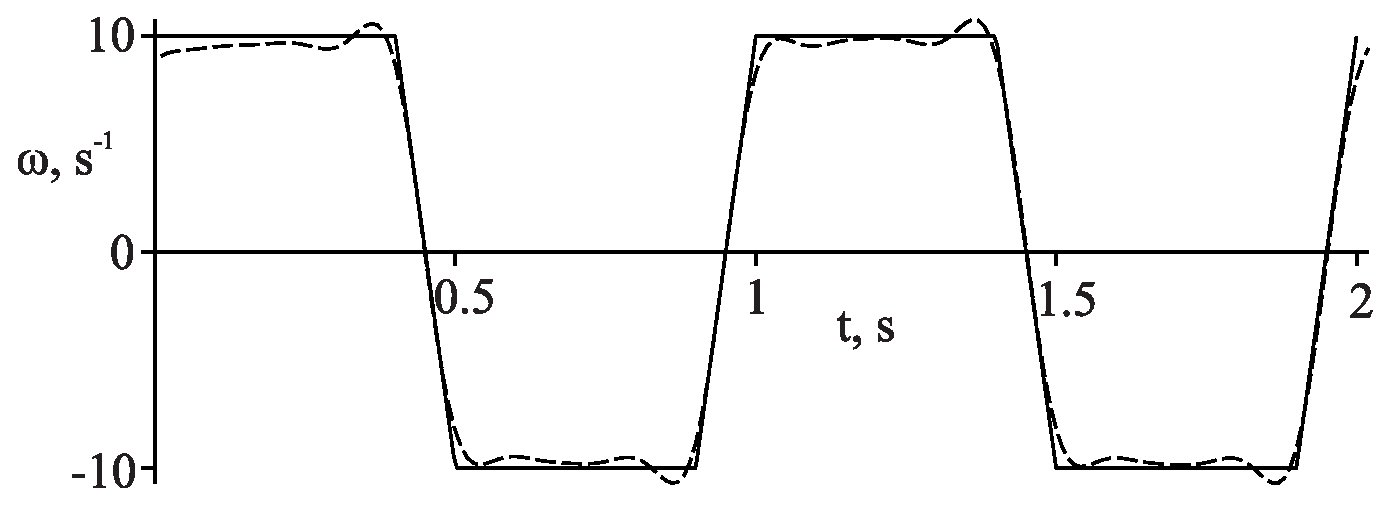
\includegraphics[width=0.9\linewidth]{OmegaT1Meandr.eps} \\ a}
	\end{minipage}
	\hfill
	\begin{minipage}[h]{0.5\linewidth}
		\center{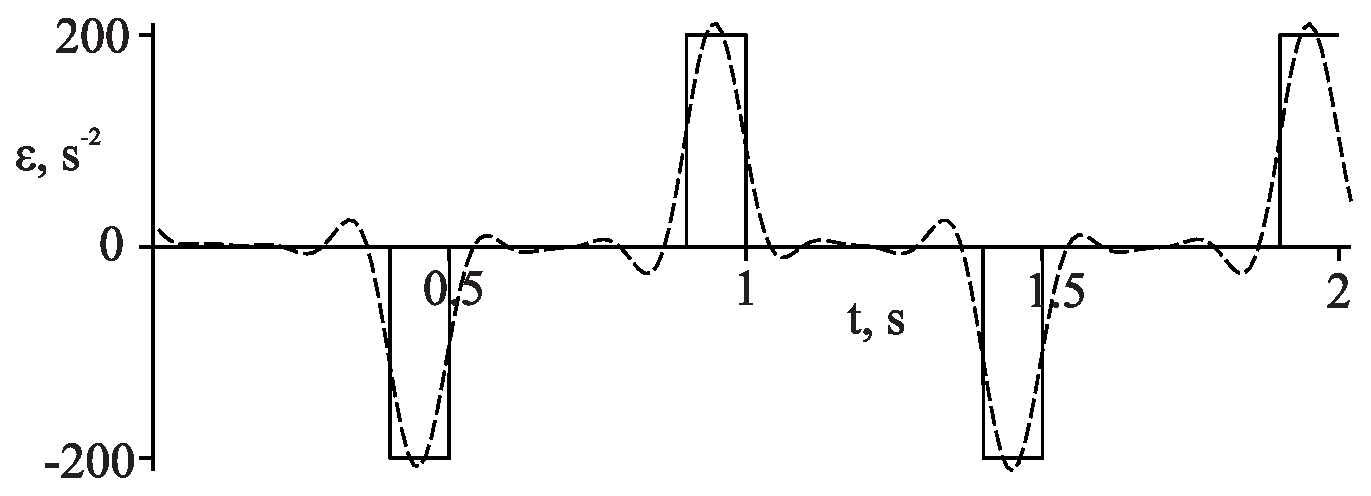
\includegraphics[width=0.9\linewidth]{EpsilonT1Meandr.eps} \\ b}
	\end{minipage}
	\caption{Зависимость угловой скорости ротора (a) и углового ускорения ротора (b) от времени при эксперименте (штриховая линия) и моделировании (сплошная линия)}
	\label{OmegaT1EpsilonT1}
\end{figure}

%\begin{figure}[!ht]
%	\centering
%	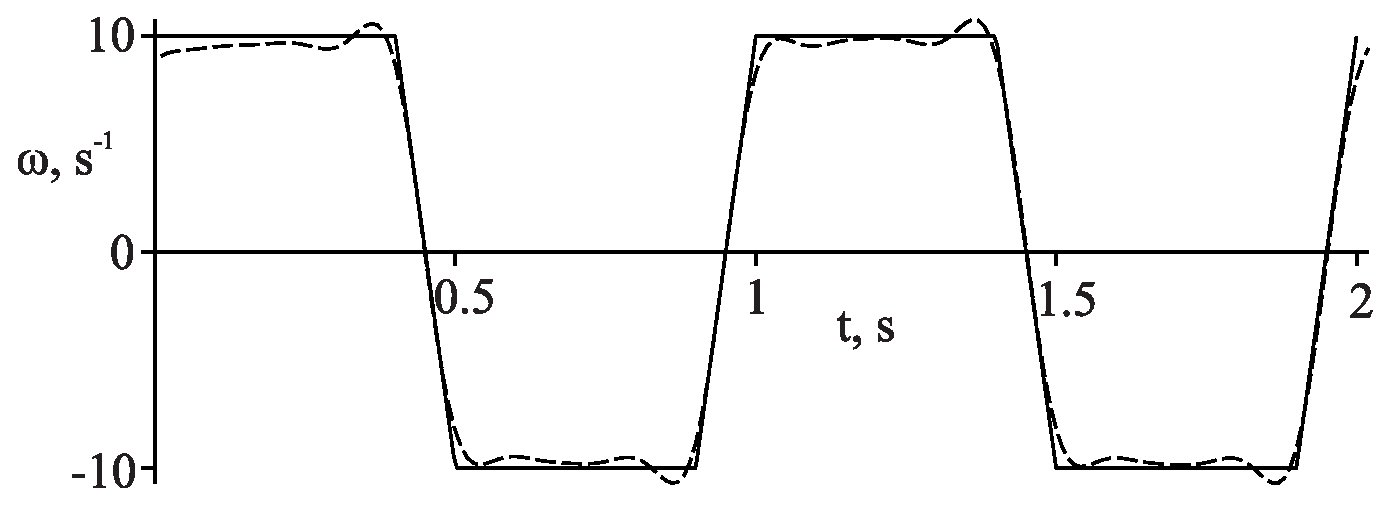
\includegraphics{OmegaT1Meandr.eps}\hspace{10mm}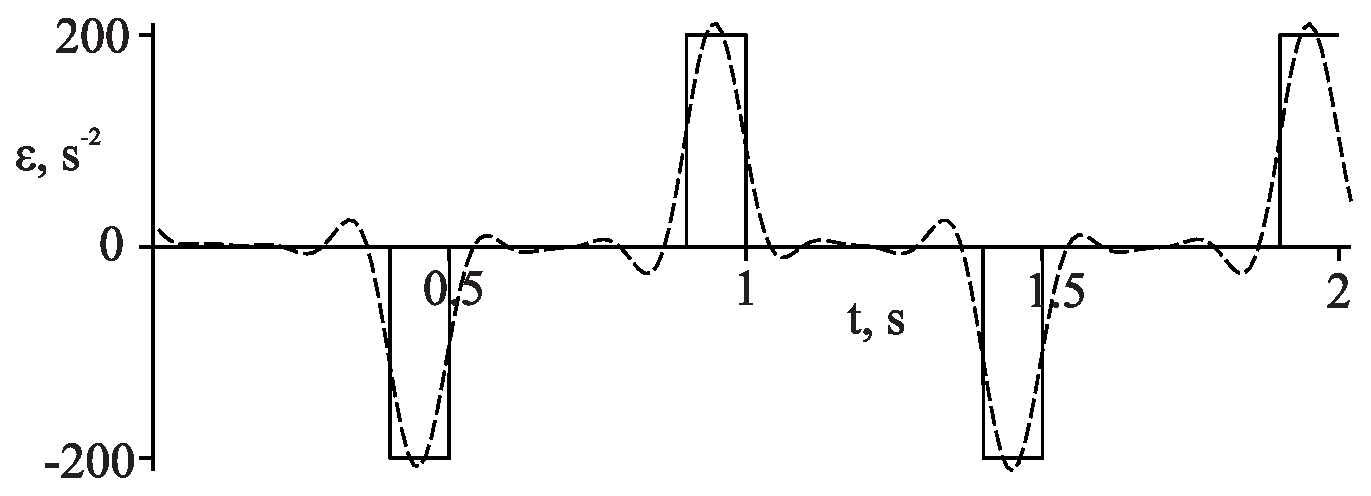
\includegraphics{EpsilonT1Meandr.eps}
%	\caption{Зависимость угловой скорости ротора (a) и углового ускорения ротора (b) от времени при эксперименте (штриховая линия) и моделировании (сплошная линия)}
%	\label{OmegaT1EpsilonT1}
%\end{figure}

Данную причину возможно устранить при использовании более моментных двигателей, более дорогих и точных в исполнении механических передач, исключающих люфт, а также более точных датчиков обратной связи.

Кроме того, повысить маневренность и управляемость движения водного робота можно добиться при модификации управляющего воздействия, обеспечив на интервалах $t_2,t_4 $ вращение ротора с разными ускорениями после смены направления вращения (см. рисунок \ref{gen_cont_ac}).    

\begin{figure}[!ht]
	\centering
	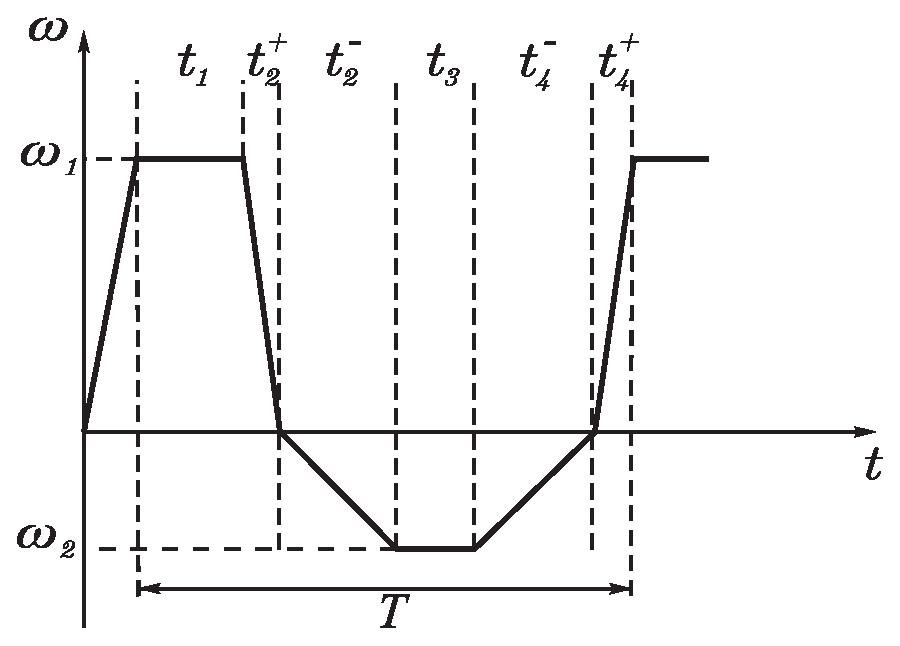
\includegraphics[width=0.5\linewidth]{ControlActionGeneral.eps}
	\caption{Общий вид управляющего воздействия при различных ускорениях разгона и торможения}
	\label{gen_cont_ac}
\end{figure}

%В дальнейшем планируется провести исследования коэффициентов от режимов и параметров движения водного робота, в том числе для случаев трехмерного движения. Также планируется разработка конструкции подводного робота, реализующего подобный принцип передвижения в жидкости.


\clearpage